\section*{Introdução}

\begin{frame}
	\frametitle{Conteúdo}
	\tableofcontents[pausesections]
\end{frame}

% -------------------------------- section ------------------------------------
\section{Empreendedorismo}

% -------------------------------- frame ----------------------------------

\begin{frame}
    \frametitle{Plano de negócios}


\begin{figure}[!h]
	\begin{center}
		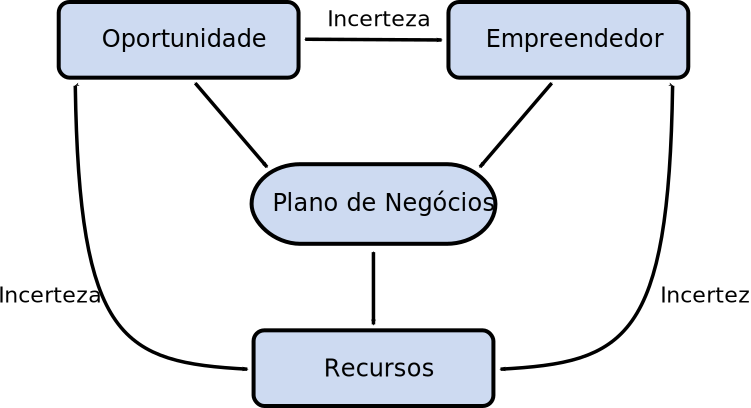
\includegraphics[scale=0.5]{imagens/componentes.pdf}
	\end{center}
	\caption{O relacionamento dos três componentes, baseado no 
		\textit{framework} de Jeffry Timmons (TIMMONS; SPINELLI, 2004).}			
\end{figure}

\end{frame}

% -------------------------------- frame ----------------------------------

\begin{frame}
    \frametitle{Estratégia competitiva}


\begin{figure}[!h]
	\begin{center}
		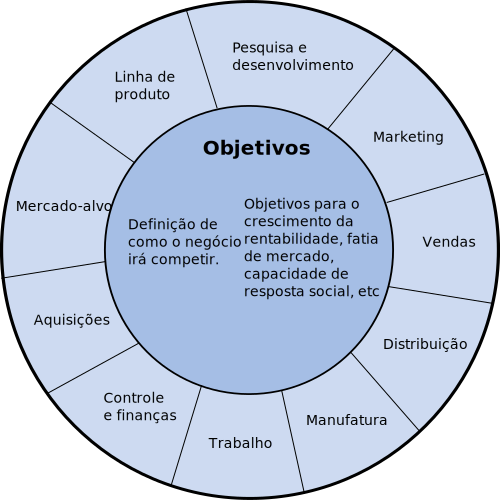
\includegraphics[scale=0.5]{imagens/estrategia.pdf}
	\end{center}
	\caption{A roda da estratégia competitiva (TIMMONS; SPINELLI, 2004) (SLACK; CHAMBERS; JOHNSTON, 2009).}			
\end{figure}

\end{frame}

